\section{Vernetzung}
Mit neuen Anforderungen an die Sicherheit und Effizienz, sowie einer Vielzahl von gewünschten Features 
für Komfort und Unterhaltung, zeichnet sich ein enormer Anstieg der in modernen Fahrzeugen verbauten ECUs (Electronic Control Unit) ab \cite{TW_kim2014gateway}.
Ein Großteil dieser Systeme und Steuergeräte ist voneinander abhängig. Zentral erfasste Signale werden von mehr als nur einem
System benötigt und verarbeitete Signale, sowie berechnete Werte müssen zwischen zusammenhängenden Systemen vermittelt werden.

Mit einer herkömmlichen Verkabelung der einzelnen Komponenten wie zu Beginn der Automobilindustrie ist ein derartiges Wachstum
nicht zu bewältigen \cite{leen1999digital}. Neben Problemen wie erhöhtes Gewicht und Kosten einer solchen Verkabelung, bietet ein solches System kein flexiblen modularen Aufbau (Composability) \cite{reif2011bosch}. Dies hat zur Folge, dass neue Teilkomponenten nicht in das Gesamtsystem integriert werden können, ohne die Funktion 
weiterer Teilkomponenten zu beeinflussen. Somit ist ein modularer Aufbau des internen Kommunikationsnetzwerkes eines Fahrzeugs nötig, um die 
steigende Komplexität der verbauten Elektronik zu bewältigen \cite{reif2011bosch}.

Im Hinblick auf die erhöhte Komplexität der Elektronik als Folge von stetig wachsenden Anforderungen werden wir im Folgenden
einen Überblick über die Topologie, verwendete Technologien und Netzwerkprotokolle, sowie die Unterteilung und Kopplung des internen Netzwerks eines Fahrzeugs bieten.

    \subsection{Topologie}
    Die Topologie eines Netzwerkes spiegelt die Anordnung der Knoten und Leitungen des Netzwerks wieder. Sie bildet ab, in welcher Weise Daten zwischen
    den einzelnen Knoten ausgetauscht werden können. Je nach Anforderungen an das Netzwerk werden unterschiedliche Topologien verwendet,
    welche einen weitreichenden Einfluss auf die Eigenschaften des Teilnetzwerkes und des Gesamtsystems haben.
        \begin{itemize}
            \item \textbf{Ringtopologie}: Hier sind die Netzwerkknoten in einem Ringschluss verbunden. Der Zugriff auf das Medium erfolgt typischerweise sequentiell 
            oder mittels eines Tokens. Es gibt sowohl unidirektionale als auch bidirektionale Ringstrukturen. Bei letzterem existiert ein gegenläufiger Ring, 
            so dass beim Ausfall einer Station nicht das gesamte Netzwerk betroffen ist. FDDI etwa ist ein derartiger Dual-Ring.
            \item \textbf{Sterntopologie}: Bei dieser Topologie sind die einzelnen Knoten mit einem zentralen Knoten verbunden. Der Ausfall eines Links beeinflusst lediglich
            eine Station, durch den zentralen Knoten existiert jedoch ein Single-Point-Of-Failure. Sterntopologien sind sehr gut skalierbar und werden oft in größeren Netzwerken eingesetzt.
            \item \textbf{Maschentopologie}: Hierbei werden die Knoten des Netzwerks direkt miteinander verbunden. In einem vollvermaschten Netz besitzt jeder Knoten eine 
            dedizierte Verbindung zu allen anderen Knoten im Netzwerk. Vorteile sind hohe Ausfallsicherheit und schnelle Datenübertragung. Jedoch steigt die Anzahl der 
            nötigen Verbindungen in einem vollvermaschten Netzwerk quadratisch mit der Anzahl an Knoten an.
            \item \textbf{Bustopologie}: Bei dieser Topologie sind alle Knoten mit einem einzigen Übertragungsmedium verbunden. Fällt eine Station aus, so ist der Rest des Netzwerks
            nicht betroffen. Da mehrere Stationen auf ein Medium zugreifen, kommen entsprechende Zugriffsverfahren zum Einsatz. Vorteile sind etwa geringe Kosten und die
            einfache Erweiterung um neue Knoten.
            \item \textbf{Hybridtopologie}: Oftmals sind auch hybride Varianten der genannten Topologien anzutreffen. Beispielhaft ist eine Stern-Ring-Topologie denkbar, indem
            mehrere Ringe über einen zentralen Hub oder Switch verbunden werden.
        \end{itemize}
    \subsection{Zugriffsverfahren}
    Für unterschiedlich verwendete Technologien und Anforderungen können verschiedene Zugriffsverfahren genutzt werden. Diese sind nötig um Kollisionen bei gleichzeitigem
    schreibenden Zugriff, durch mehrere Knoten eines Netzwerks auf das selbe Übertragungsmedium zu verhindern. Im Folgenden werden einige Möglichkeiten kurz dargestellt.
        \begin{itemize}
            \item \textbf{TDMA}: Time Division Multiple Access ist ein Verfahren, bei dem die Zugiffszeit in Zeitslots unterteilt wird, welche den entsprechenden
            Stationen des Netzwerks zugeordnet werden. Dadurch können Kollisionen vermieden werden, indem Knoten nur in den ihnen zugeteilten Zeitslots Signale 
            senden. Bei geringer Auslastung ist ein derartiges Verfahren jedoch suboptimal, da die Gesamtzugriffszeit nicht effektiv ausgenutzt werden kann.
            \item \textbf{FDMA}: Frequency Division Multiple Access ist ein Multiplexingverfahren bei dem die verfügbare Bandbreite in nicht-überlappende Frequenzbereiche aufgeteilt wird,
            um das Senden von Daten durch mehrere Knoten zum selben Zeitpunkt zu ermöglichen.
            \item \textbf{CDMA}: Code Division Multiple Access ist eine Form von Multiplexing, welche erlaubt, dass mehrere Teilnehmer gleichzeitig im selben Frequenzbereich
            senden können. Hierfür werden Spreizcodes verwendet, welche ermöglichen, dass mehrere Stationen zur selben Zeit unterschiedlich codierte Daten senden können.
            Anhand dieser Codierung können die Datenströme bei den Empfängern wieder herausgerechnet werden.
            \item \textbf{Token Passing}: Hierbei handelt es sich um ein Zugriffsverfahren welches etwa bei Token-Ring oder FDDI zum Einsatz kommt. Die Sendeerlaubnis ist bei diesem
            Verfahren abhängig vom Besitz eines authoritativen Tokens, welches innerhalb des Netzwerks weitergereicht wird.
            \item \textbf{CSMA/CD}: Carrier Sense Multiple Access / Collision Detection ist ein Zugriffsverfahren, welches bei Ethernet Anwendung findet. Dabei lauschen teilnehmende Stationen
            auf dem gemeinsam genutzten Medium auf Übertragungen. Ist das Medium frei, können Daten gesendet werden. Hierbei lassen sich Kollisionen jedoch nicht vermeiden, sondern lediglich 
            erkennen. 
            
            Sobald während des eigenen Sendevorgangs weitere Signale ausgehend von einer anderen Quelle erkannt werden, wird die Übertragung abgebrochen. Anschließend wird ein
            Jamming-Signal ausgesendet und eine gewisse Zeitspanne gewartet, bevor der Prozess erneut beginnt (Lauschen auf Belegung des Mediums, Sendeversuch und Kollisionserkennung).
            Aufgrund der Etablierung von Switched Ethernet und der entstehenden kollisionsfreien Domänen wird CSMA/CD kaum noch benötigt. Im WLAN wird CSMA/CA verwendet.
        \end{itemize}
    \subsection{Kommunikation}
    Die eigentliche Datenkommunikation in einem Netzwerk kann anhand der Adressierungsart, sowie verwendeten Steuermechanismen unterschieden werden. 

    So ist die am häufigsten vorzufindende Adressierungsart teilnehmerorientert. Grundlage dieser Form des Datenaustauschs sind Knotenadressen, welche zusammen mit den
    zu übertragenden Daten die eigentliche Nachricht bilden \cite{reif2011bosch}. Diese Form der Adressierung findet man etwa bei Ethernet oder IP. 

    Eine weitere Adressierungsart, welche im Kontext des Automobils von Relevanz ist, ist die nachrichtenorientierte Adressierung. Hierbei werden nicht Empfänger, sondern die Nachrichten selbst
    adressiert, indem sich ein Identifier in den Nachrichten befindet, welcher den Nachrichtentyp kennzeichnet \cite{reif2011bosch}. In diesem Fall benötigt der Sender keine 
    Kenntnisse über Teilnehmer bzw. deren Adressen und jeder Empfängerknoten entscheidet selbstständig ob er eine Nachricht verarbeitet \cite{reif2011bosch}. Später betrachtete
    Protokolle wie CAN, LIN und Flexray sind Beispiele für nachrichtenorientierte Protokolle.

    Auch Anhand der Steuermechanismen kann die Kommunikation in Netzwerken unterschieden werden. Unterschieden wird zwischen ereignis- und zeitgesteuerten Systemen.

    Ereignisgesteuerte Bussysteme können aufgrund der inhärent fehlenden Synchronisation der Nachrichten und folglich entstehenden Kollisionen beim Zugriff auf den Bus
    überlastet werden, sollte die Anzahl der interagierenden Knoten zu hoch sein \cite{reif2011bosch}. Besonders gut geeignet sind derartige Systeme für unerwartete Ereignisse,
    welche idealerweise ohne Latenz im Vergleich zu zeitgesteuerten Systemen übertragen werden können \cite{reif2011bosch}. Beispielhaft hierfür sind jegliche Interaktionen eines 
    Fahrzeugführers mit dem System. Bei erhöhten Anforderungen bezüglich der Sicherheit und Zuverlässigkeit eines Systems bieten sich wiederum zeitgesteuerte Systeme an \cite{reif2011bosch}.
    Elektronische Brems- und Lenksysteme benötigen derartige zeitliche Zusicherungen.
    \subsection{Technologie}
    Nachdem wir einige grundsätzliche Aspekte und Terminologien bezüglich der Vernetzung und Kommunikation betrachtet haben, geben wir im folgenden einen kurzen Überblick
    über verwendete Technologien und Netzwerkprotokolle, welche wir je nach Relevanz in einer späteren Sektion noch einmal aufgreifen und genauer betrachten werden.
        \subsubsection{Wired}
        Im folgenden geben wir einen Überblick über die am meisten verbreitetsten Netzwerkprotokolle in heutigen Fahrzeugen. 
            \begin{itemize}
                \item \textbf{CAN} (Controller Area Network): CAN wird seit langer Zeit für den Großteil der Datenkommunikation in Fahrzeugen verwendet \cite{leen1999digital}.
                Vor allem im Bereich des Antriebsstrangs, des Fahrwerkes sowie den Systemen zur Kontrolle des Innenraums ist CAN als bevorzugte Netzwerktechnologie vorzufinden.
                CAN ist ein asynchroner serieller Bus-Standard, welcher Steuergeräte, Sensoren und Aktoren zu einem System verbindet. 
                
                Es handelt sich um ein Multi-Master Kommunikationsprotokoll, welches für Datenintegrität und Automobilapplikationen mit Datenraten von bis zu 1 MB/s geschaffen wurde \cite{wolf2004security}. Vorteile
                dieser Technologie sind die geringen Kosten und die hohe Zuverlässigkeit. Eingeschränkt ist die Technologie durch die geringe Bandbreite, weshalb Sie
                ungeeignet für Unterhaltung und Medienstreams ist \cite{TW_huang2018vehicle}.
                \item \textbf{LIN} (Local Interconnect Network): LIN ist ein asynchrones, single-master, multi-slave Netzwerkprotokoll, welches in Hinblick auf Kostenersparnis 
                designed wurde. Eingesetzt wird LIN vor allem für Low-Speed-Kommunikation und stellt eine kosteneffiziente Alternative dar, um Motor und Sensoren innerhalb 
                eines Fahrzeugs zu verbinden. Typischerweise kommt es bei der Elektronik des Innenraums zum Einsatz, wenn die Bandbreite von CAN nicht benötigt wird, wie z.B bei Fensterheber
                oder der Sitzanpassung \cite{TW_huang2018vehicle}.
                \item \textbf{Flexray}: Flexray wurde als eine schnellere, zuverlässige aber auch teurere Alternative zu CAN entwickelt. Es handelt sich um ein Kommunikationsprotokoll mit einer
                Dual-Channel Datenrate von bis zu 10 MB/s für komplexere Kontrollsysteme innerhalb eines Fahrzeugs \cite{wolf2004security}. Über die Dual-Channel Architektur kann die Zuverlässigkeit
                bei Anwendungen wie Brake-By-Wire gewährleistet werden \cite{TW_huang2018vehicle}. 
                \item \textbf{MOST} (Media Oriented Systems Transport): MOST ist eine High-Speed Netzwerk Spezifikation, welche speziell für Übertragung von Medien wie Audio und Videosignalen 
                geschaffen wurden. Es handelt sich dabei um einen seriellen Bus welcher eine Ringtopologie verwendet \cite{TW_huang2018vehicle}.
                \item \textbf{Ethernet}: Als Standardtechnologie für drahtgebundene lokale Netzwerke spielt Ethernet eine kritische Rolle bei jeglicher Art von Kommunikation.
                Vorteile von Ethernet als Mittel zur Vernetzung gegenüber bereits genannten Technologien sind die deutlich höhere Bandbreite, Skalierbarkeit und Flexibilität \cite{hank2013automotive}\cite{TW_huang2018vehicle}. 
            \end{itemize}
        \subsubsection{Wireless}
        Als alternatives Mittel zur herkömlichen verdrahteten Kommunikation zwischen den Komponenten eines Fahrzeugs existieren auch einige drahtlose Technologien.
        Diese können nicht nur zur Verbindung zwischen persönlichen Geräten des Fahrers mit dem Fahrzeug, sondern auch zur Verbindung der internen Systeme genutzt werden.
        Damit könnte ein Großteil der Sensoren, Aktoren und ECUs drahtlos verbunden werden.
            \begin{itemize}
                \item \textbf{WLAN}: Der Standard IEEE 802.11 wurde als drahtlose Alternative zu kabelgebunden High-Speed
                Netzwerken geschaffen. Auch im Automobil kann WLAN genutzt werden um persönliche Geräte wie Smartphones,
                Tablets und Laptop mit dem Unterhaltungssystem des Fahrzeugs zu verbinden \cite{TW_huang2018vehicle}. 
                \item \textbf{Bluetooth}: Bluetooth wurde für drahtlose Kurzstrecken-Kommunikation designed. Optimiert wurde die
                Technologie für Audiostreams und ist idealerweise für drahtlose Lautsprecher eines mobilen Audiosystems geeignet.
                Auch händefreies Telefonieren über eine Verbindung zum Smartphone ist bereits im Großteil der modernen Fahrzeuge 
                über Bluetooth möglich.
                
                BLE (Bluetooth Low Energy 4.0) ermöglicht Verbindungen mit geringer Latenz, hoher Zuverlässigkeit
                und geringem Energieverbrauch, weshalb der Einsatz dieser Technologie zur Verbindung von Sensornetzwerken und ECUs im Innenraum, 
                dem Antriebsstrang und Fahrwerk denkbar wäre \cite{TW_huang2018vehicle}. Für kritische Systeme wie Brems- und Lenksysteme bleibt der Einsatz jedoch bedenklich \cite{wolf2004security}.
                \item \textbf{UWB} (Ultra-Wideband): UWB ist eine Radiowellen Technologie für kurze Entfernung und hohe Bandbreite, welche als Alternative zu Wifi und Bluetooth gesehen werden kann.
                \item \textbf{Zigbee}: Zigbee ist ein kabelloser Standard, welcher auf dem Standard IEEE 802.15.4 beruht und Geräte mit geringerem Datendurchsatz und niedrigem Energieverbauch in einem 
                Mesh-Netzwerk verknüpft. Die Datenraten reichen bis zu 250 KB/s. Zigbee kann genutzt werden um ECUs, Sensoren und Aktoren in einem Fahrzeug zu verbinden \cite{TW_huang2018vehicle}.
            \end{itemize}
    \subsection{Systemunterteilung}
    Mit dem Einzug einer Vielzahl neuer Systeme für die Unterhaltung, Navigation, On-Board Diagnostik,
    Augmented Reality (AR) Dashboards oder etwa Fahrassistenzsysteme finden wir in aktuellen Top-Modellen bereits 
    ca. 70 ECUs \cite{TW_huang2018vehicle}. Mit steigender Anzahl und zunehmender Komplexität 
    benötigen diese ECUs eine größere Bandbreite und geringere Latenz des internen Netzwerks \cite{TW_huang2018vehicle}.
    Das Gesamtsystem lässt sich hierbei in die 4 Bereiche Powertrain, Chassis, Innenraum und Telematik/Infotainment unterteilen.
        \subsubsection{Powertrain}
        Der Antriebsstrang umfasst alle Komponenten welche für die Leistungserzeugung für den Antrieb verantwortlich sind. Dies umfasst 
        den Motor, Getriebe, Antriebswelle, Räder etc. Von Relevanz sind hierbei etwa die Engine Control Unit oder das Powertrain Control Module.
        Auch Sensoren und Aktoren, etwa zur Erhebung und Regulation von Geschwindigkeit, Drehzahl, Öl-Stand, Zylinderdruck, Position, Stabilität sind hierbei miteinbegriffen.
        Im Bereich des Antriebstrangs stehen Echtzeitanwendungen im Vordergrund \cite{reif2011bosch}\cite{TW_huang2018vehicle}.
        \subsubsection{Chassis}
        Das Fahrwerk umfasst alle Komponenten welche den Antriebsstrang und die Karosserie tragen. Bekannte Komponenten sind etwa
        Bremsen, Lenkung und Federung. Hier finden wir eine Vielzahl von Sensoren und Aktoren etwa für das ABS (Anti-Lock Braking System) und ESP (Electronic Stability Program).
        Wie auch beim Antriebsstrang sind hohe Datenraten für das gewünschte Echtzeitverhalten nötig \cite{TW_huang2018vehicle}.
        \subsubsection{Innenraum}
        Der Innenraum setzt sich aus einer Reihe von Teilsystemen zusammen. Hierzu gehören die meisten Komfort-Systeme wie etwa Klimaregelung, Sitz- und Spiegelanpassung, Fensterheber, Beleuchtung,
        Anzeige, Scheibenwischer, aber auch Zugangsberechtigung und Diebstahlwarneinrichtung \cite{reif2011bosch}. 
        Diese benötigen meist nur eine geringe Bandbreite und haben eine hohe Toleranz für zeitliche Verzögerungen.
        \subsubsection{Telematik und Infotainment}
        Dieses Teilsystem umfasst alle Schnittstellen zur Interaktion zwischen Mensch und verbauter Elektronik. So können etwa Informationen welche über Sensoren
        oder ECUs gewonnen wurden in einer interaktiven Weise dem Nutzer zu Unterhaltungszwecken dargestellt werden \cite{TW_huang2018vehicle}.
        
        Auch die Interaktion von Mobilgeräten
        zum Zwecke der Unterhaltung, Kontrolle oder Wartung von Systemen zählt hierzu. Beispiele wären Autoradio, Navigationssystem, Video- und Sprachanlage, Rückfahrkamera und Fahrerinformationssysteme \cite{reif2011bosch}.
        Meist benötigen diese Teilsysteme eine hohe Bandbreite, tolerieren aber einen gewissen Grad an Verzögerung.
    \subsection{Systemkopplung}
    Aufgrund der unterschiedlichen Anforderungen der Teilsysteme eines Fahrzeugs, etwa an Echtzeitverhalten, Zuverlässigkeit und Fehlertoleranz werden unterschiedliche Technologien
    und Netzwerktopologien mit angemessenen Vor- und Nachteilen verwendet \cite{leen1999digital}. 
    
    Da diese Technologien meist nicht kompatibel zueinander sind, können Daten nicht ohne Weiteres zwischen diesen
    Teilsystemen ausgetauscht werden. In der Regel ist hierbei ein Gateway zwischengeschaltet, welches Daten eines Protokolls einliest und das Format entsprechend des Zielsystems anpasst
    und weitersendet \cite{reif2011bosch}\cite{TW_kim2014gateway}. Hierbei kann ein zentrales (Abb. 1 (a)) oder aber mehrere verteilte Gateways (Abb. 1 (b)) genutzt werden. 

    In Abb. 1 (a) sehen wir einen beispielhaften Aufbau eines internen Netzwerks, verknüpft über ein zentrales Gateway. Aufgrund der Echtzeitanforderungen und Zuverlässigkeit wird in diesem Fall Flexray
    im Chassis Teilsystem verwendet. Die Steuergeräte des Antriebsstrangs sind wiederum über ein CAN Bus der Klasse C (High-Speed-CAN) verbunden. Das System des Innenraums verwendet in diesem Fall 
    CAN-B (Low-Speed-CAN), da die Echtzeitanforderung bei den Komfortfunktionen entfällt. Im Bereich der Telematik wird aufgrund der benötigten Bandbreite MOST eingesetzt. Einzelne Systeme welche die
    Bandbreite von CAN nicht benötigen, können mit LIN ebenfalls über das Gateway mit dem Gesamtsystem verknüpft werden.
    Abb. 1(b) spiegelt einen Aufbau mittels mehrerer Gateways wieder.

    \begin{figure}
    \caption{Netzwerk mit (a) zentralem Gateway und (b) mehreren Gateways \cite{reif2011bosch}}
    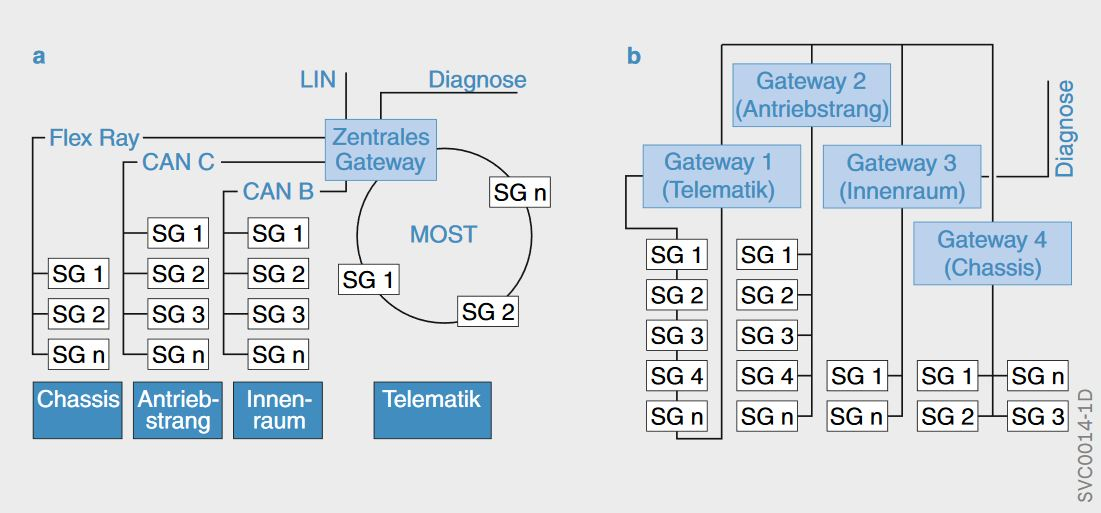
\includegraphics[width=\textwidth]{Images/Kapitel3/TW01.JPG}
    \end{figure}
